\autobookmark
\begin{frame}{Distribution of rays on a GPU}
  \begin{columns}[T]

    \begin{column}{.4\textwidth}
      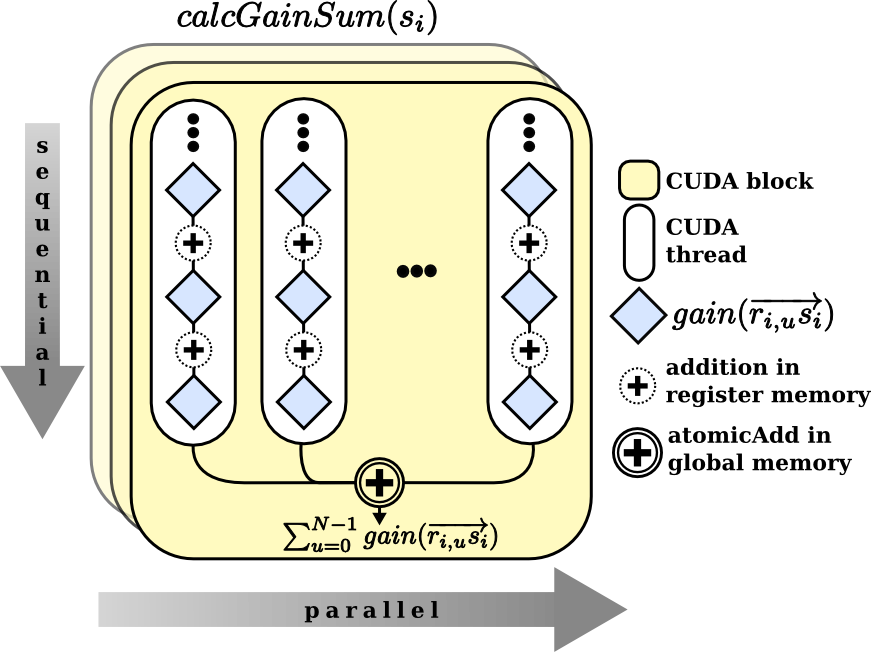
\includegraphics[width=0.4\paperwidth]{graphics/kernel_detail5.png}
    \end{column}

    \begin{column}{.6\textwidth}
      \begin{itemize}
          \myuncover{1}{4}{
          \item A CUDA thread proceses multiple rays
          \item Reduction over all threads by atomicAdd is the only synchronized part
          }
          \myuncover{2}{4}{
          \item Rays starting in similar positions are grouped together to improve caching
          }
          \myuncover{3}{4}{
          \item Importance sampling distributes rays in the material towards areas of interest
          }
          \myuncover{4}{4}{
          \item Load balancing between blocks, to reduce impact of different ray lengths
          }
      \end{itemize}
    \end{column}


  \end{columns}

\end{frame}

%\begin{frame}{Predefined colours}
%  The template defines a set of colours according to the CD guidelines:\par
%  \begin{itemize}
%      \begin{minipage}[t]{0.5\linewidth}
%      \item \textcolor{hzdr-blue}{Helmholtz Blue}    
%      \item \textcolor{hzdr-orange}{Rossendorf Orange}  
%      \item \textcolor{hzdr-darkblue}{Helmholtz Dark Blue}
%      \item \textcolor{hzdr-gray1}{Gray1}   
%      \item \textcolor{hzdr-gray2}{Gray2}   
%      \item \textcolor{hzdr-gray3}{Gray3}   
%      \item \textcolor{hzdr-struct}{Structure of Matter}  
%      \end{minipage}%
%      \begin{minipage}[t]{0.5\linewidth}
%      \item \textcolor{hzdr-health}{Health}  
%      \item \textcolor{hzdr-energy}{Energy}  
%      \item \textcolor{hzdr-earth}{Earth and Environment}   
%      \item \textcolor{hzdr-keytec}{Key Technologies}  
%      \item \textcolor{hzdr-aero}{Aeronautics, Space and Transport}
%      \end{minipage}
%  \end{itemize}
%\end{frame}

